\documentclass[manuscript,review,anonymous]{acmart}

%% ------------------------------------------------------------------
%% BASiS: Bayesian Style-based Selection
%% IUI 2027 double-blind submission draft
%% Compile with pdflatex (or latexmk -pdf) + bibtex.
%% ------------------------------------------------------------------

\usepackage{amsmath}
\usepackage{booktabs}
\usepackage{graphicx}
\usepackage{tabularx}
\usepackage{array}
\usepackage{comment}

%% Uncomment once the submission ID has been issued by PCS.
%% \acmSubmissionID{123-A45-B67}

\setcopyright{acmlicensed}
\acmConference[IUI '27]{32nd Annual ACM Conference on Intelligent User Interfaces}{February 8--11, 2027}{Helsinki, Finland}
\acmDOI{}
\acmISBN{}

\begin{document}

\title{BASiS: Adapting Conversational Behavior in Purpose-Specific Dialogue Systems through Bayesian Data Selection}

\author{Anonymous Author(s)}
\affiliation{%
  \institution{Institution withheld for review}
  \city{City}
  \country{Country}
}
\renewcommand{\shortauthors}{Anonymous Author(s)}

\begin{abstract}
We propose BASiS (Bayesian Style-based Selection), a method that treats a small, high-quality dialogue corpus not merely as a collection of utterances, but as a source of implicit knowledge about how conversations unfold. BASiS models this knowledge through transitions among dialogue states and probability distributions over response strategies, then repurposes the model as a criterion for selecting training data from a large general-purpose corpus. We focus on settings where dialogue must progress according to the user’s state and interactional phase. In such settings, dialogue quality depends not only on utterance content, but also on procedural interactional knowledge: how to interpret the user’s situation and which dialogue strategy to use at what point. Although such knowledge is implicitly encoded in small, high-quality corpora, these corpora alone provide limited data for LLM training. BASiS extracts dialogue states, response strategies, and state transitions from the small corpus and represents them as a Bayesian dialogue model. It then scores dialogues in a large corpus by their compatibility with the target conversational style, selects training data, constructs preference pairs, and trains the LLM using Direct Preference Optimization (DPO). This uses knowledge from limited high-quality dialogues to guide training-data expansion. It also reduces the need for manually designed dialogue guidelines while incorporating response timing and multi-turn progression that generic quality or topical similarity cannot capture. By maintaining dialogue states probabilistically rather than choosing a single response strategy, BASiS can preserve multiple valid strategies for the same context. We evaluated BASiS in emotional support, mathematics tutoring, and medical interviewing against the base model and a model trained on randomly selected in-category data. BASiS achieved the highest mean score on all 21 evaluation dimensions, with broad statistically significant improvements in emotional support and mathematics tutoring.
\end{abstract}

\begin{CCSXML}
<ccs2012>
 <concept>
  <concept_id>10010147.10010178.10010179</concept_id>
  <concept_desc>Computing methodologies~Natural language generation</concept_desc>
  <concept_significance>500</concept_significance>
 </concept>
 <concept>
  <concept_id>10010147.10010178.10010179.10010182</concept_id>
  <concept_desc>Computing methodologies~Discourse, dialogue and pragmatics</concept_desc>
  <concept_significance>500</concept_significance>
 </concept>
 <concept>
  <concept_id>10003120.10003121.10003122.10003334</concept_id>
  <concept_desc>Human-centered computing~Natural language interfaces</concept_desc>
  <concept_significance>300</concept_significance>
 </concept>
 <concept>
  <concept_id>10010147.10010257.10010293.10010294</concept_id>
  <concept_desc>Computing methodologies~Learning from implicit feedback</concept_desc>
  <concept_significance>100</concept_significance>
 </concept>
</ccs2012>
\end{CCSXML}

\ccsdesc[500]{Computing methodologies~Natural language generation}
\ccsdesc[500]{Computing methodologies~Discourse, dialogue and pragmatics}
\ccsdesc[300]{Human-centered computing~Natural language interfaces}
\ccsdesc[100]{Computing methodologies~Learning from implicit feedback}

\keywords{purpose-specific dialogue systems, conversational style, data selection, Bayesian dialogue modeling, preference optimization, emotional support dialogue, large language models}

\maketitle

\section{Introduction}
\label{sec:intro}

Advances in instruction tuning and reinforcement learning from human feedback (RLHF) have enabled recent large language models (LLMs) to follow instructions, generate accurate responses, and sustain natural and coherent multi-turn conversations across a wide range of topics \cite{ouyang2022instructgpt}. In purpose-specific dialogue such as emotional support, mathematics tutoring, and medical history-taking, however, a system must do more than provide correct information: it must choose an appropriate response policy based on the interlocutor's state and the current stage of the dialogue \cite{rashkin2019empathetic,liu2021esconv}. For example, it may need to acknowledge a person's feelings before offering advice, encourage a learner to reason independently, or elicit necessary symptoms in an appropriate order. Such conversational styles are reflected in small, high-quality corpora developed for specific purposes, but these corpora are limited in size for direct use in LLM training. Large general-purpose corpora offer greater volume and diversity, yet they do not necessarily include enough dialogues that match the target style. A method is therefore needed to incorporate the dialogue progression captured in a small, high-quality corpus into the responses actually generated by an LLM.

Several approaches have been explored to generate responses suited to purpose-specific dialogue. Guideline-based response control explicitly defines a desirable dialogue policy in advance and guides response generation to follow it. GuidedTOD, proposed by Wen et al., probabilistically represents the flow of task-oriented dialogue and reranks candidate responses while updating a guideline-based policy as the dialogue progresses; it achieved higher guideline compliance than previous methods \cite{wen2025guidedtod}. Other work predicts the next dialogue action or response strategy from dialogue history. Ganesh et al. predicted the next teacher talk move in classroom dialogue \cite{ganesh2021teacher}; Wan et al.'s EmoDynamiX modeled relationships between multiple user emotion states and response strategies as a heterogeneous graph \cite{wan2025emodynamix}; and Rudolph et al. regularized next-dialogue-act prediction using a transition matrix derived from counseling conversations \cite{rudolph2026transition}. Research on selecting LLM training data has further shown that carefully chosen, high-quality data can efficiently adapt model behavior even when the selected dataset is small \cite{zhou2023lima,zhang2025datasurvey}.

These approaches nevertheless leave two challenges. First, guideline-based response control requires desirable dialogue policies to be written manually for each purpose or domain. Conversational style is often expressed implicitly through tone, response timing, and progression across multiple turns, making it difficult to describe comprehensively as explicit rules. Second, existing work on dialogue actions and response strategies primarily models dialogue flow to predict the next action or strategy; it does not extend to generating natural-language responses from those predictions or evaluating the quality of the generated responses. How to incorporate dialogue structure learned from a corpus into actual response generation therefore remains underexplored.

To address these challenges, we propose BASiS (Bayesian Style-based Selection), a method that adapts a local LLM to the conversational style required for purpose-specific dialogue through Bayesian data selection based on a small, high-quality corpus. BASiS first uses an LLM to analyze the small corpus and structures each dialogue in terms of conversational states, which describe the interlocutor's situation or the stage of the dialogue; response strategies, which describe response policies such as empathy, questioning, and advice; and state transitions caused by the responses. It then constructs a Bayesian dialogue model from this structure, using transition probabilities between states and observation likelihoods for response strategies in each state. The model scores each dialogue instance in a large general-purpose corpus according to its compatibility with the target conversational style and selects data for training. Finally, BASiS constructs preference pairs from the selected data and applies Direct Preference Optimization (DPO) with Low-Rank Adaptation (LoRA) to a local LLM, thereby adapting the model to the style captured in the small corpus.

A central feature of BASiS is that it represents conversational style not as individual response expressions or detailed, manually authored guidelines, but as probabilistic transitions between conversational states and response strategies. This allows the implicit dialogue flow in the corpus to guide data selection without requiring detailed guidelines for each purpose. BASiS maintains a probability distribution over conversational states and updates it using observations derived from candidate responses, thereby incorporating the current dialogue history and the resulting state transition into data selection. Moreover, the same procedure can be applied to different purpose-specific settings, including emotional support, mathematics tutoring, and medical history-taking, by changing the small reference corpus and the large corpus from which data are selected. Using the selected data for LoRA-based DPO allows the target style to be incorporated while retaining the general dialogue capabilities of the local LLM.

The remainder of this paper is organized as follows. Section~\ref{sec:relwork} reviews related work on guideline-based response control, dialogue-history-based prediction of dialogue actions and response strategies, and training-data selection for LLMs. Section~\ref{sec:method} describes the BASiS training pipeline and the role of each module. Section~\ref{sec:evaluation} presents the experiments used to evaluate BASiS, their results, and our discussion. Finally, Section~\ref{sec:conclusion} concludes the paper.


\section{Related Work}
\label{sec:relwork}

One approach to realizing purpose-specific behavior in dialogue systems is to provide desirable response policies as natural-language guidelines and control response generation accordingly. Gupta et al. proposed DialGuide, which describes in natural language both the conversational contexts in which a guideline applies and the content that a response should include \cite{gupta2023dialguide}. DialGuide addresses guideline selection, guideline-grounded response generation, and verification that generated responses satisfy the selected guideline. Experiments on open-domain and safety-related dialogue data showed that it can generate safe and engaging responses that follow developer-provided guidelines. Wen et al. introduced a Chained Prior that represents a sequence of task-oriented dialogue guidelines as a Markov chain and proposed GuidedTOD, which updates its policy as the dialogue progresses \cite{wen2025guidedtod}. By reranking candidate responses with the Chained Prior, GuidedTOD improved guideline compliance over previous methods and increased action-prediction accuracy by approximately 20\%. These studies demonstrate the value of expressing desired behavior as explicit guidelines and incorporating them into response selection or generation.

Other studies predict the next dialogue action or response strategy from the preceding interaction instead of directly applying manually defined guidelines. Ganesh et al. introduced Future Talk Move Prediction, which predicts a teacher's next talk move from the classroom dialogue history and the preceding talk moves \cite{ganesh2021teacher}. By formulating teacher behavior as multiclass classification, their model substantially outperformed multiple baselines and exhibited patterns similar to those observed in human predictions. Wan et al. proposed EmoDynamiX, which models discourse-level relationships between fine-grained user emotion states and system response strategies as a heterogeneous graph \cite{wan2025emodynamix}. Across two emotional-support datasets, it achieved higher F1 scores and lower strategy-preference bias than previous methods, while also supporting interpretable backtracing of its predictions. Rudolph et al. incorporated a transition matrix estimated from counseling dialogues as a KL regularizer for next-dialogue-act prediction, aligning the predicted distribution with observed dialogue flow \cite{rudolph2026transition}. Their method improved macro-F1 by 9--42\% relative across multiple encoders and also improved dialogue-flow alignment.

Research on efficient LLM adaptation has also emphasized the quality and task relevance of training data rather than only its volume. LIMA showed that a small set of high-quality instruction--response examples can teach desirable response formats and conversational behavior \cite{zhou2023lima}. AlpaGasus and DEITA select data according to criteria such as quality, complexity, and diversity, achieving strong performance with less training data \cite{chen2023alpagasus,liu2024deita}. LESS further demonstrated the effectiveness of selecting examples according to their estimated influence on target-task performance \cite{xia2024less}. Together, these findings show that selecting high-quality data suited to the target is important for efficient model adaptation.

These studies have advanced response-policy control, dialogue-action and response-strategy prediction, and efficient selection of training data. Nevertheless, two challenges remain when incorporating purpose-specific conversational style into actual response generation. First, guideline-based methods such as DialGuide and GuidedTOD require desirable dialogue policies to be designed manually whenever the purpose or domain changes. Features expressed implicitly in a corpus---including tone, response timing, policy changes based on the interlocutor's state, and progression across multiple turns---are difficult to specify comprehensively as guidelines. This imposes substantial design costs. Moreover, because omitted features are unlikely to affect response control, the scope and quality of that control depend on the completeness of the guidelines. Second, existing work that models dialogue actions or response strategies primarily evaluates prediction rather than natural-language generation based on the predicted structure. Ganesh et al. output the label of the teacher's next talk move but do not generate a teacher response that realizes that move. EmoDynamiX can pass its predicted strategy to an external generator, but its reported evaluation concerns strategy-prediction F1, strategy-preference bias, and interpretability rather than the quality of generated emotional-support responses. Rudolph et al. likewise evaluate next-dialogue-act prediction and alignment with dialogue flow, explicitly leaving end-to-end integration with response generation unexplored. Dialogue structure learned from a corpus must therefore be incorporated into a response generator and evaluated at the level of the generated responses.


\section{BASiS}
\label{sec:method}

\subsection{Concept}
\label{sec:method_concept}

We propose BASiS (Bayesian Style-based Selection), which adapts a local large language model (LLM) to the conversational style required for purpose-specific dialogue through Bayesian data selection based on a small, high-quality corpus. BASiS converts the response policies and dialogue progression expressed implicitly in the small corpus into a form suitable for training a local LLM. Rather than training directly on the small corpus, it extracts conversational states, response strategies, and state transitions, constructs a probabilistic dialogue model, and uses that model as a criterion for selecting data from a large general-purpose corpus.

BASiS evaluates each dialogue instance in the large general-purpose corpus according to its compatibility with the conversational style characteristic of the target corpus. It incorporates the dialogue flow in the small corpus into the training data without requiring detailed, manually written dialogue guidelines for each purpose or domain. By maintaining the conversational state as a probability distribution rather than committing to a single state, BASiS represents settings in which multiple response strategies may be valid for the same context. The selected data are ultimately used for DPO training, which adapts the local LLM to the conversational style of the small corpus.

\subsection{BASiS Training Pipeline}
\label{sec:method_architecture}

Figure~\ref{fig:basis_architecture} shows the BASiS training pipeline. Its four modules---the \textbf{Dialogue Feature Analysis Module}, \textbf{Bayesian Dialogue Modeling Module}, \textbf{Style Compatibility Scoring Module}, and \textbf{Preference Data Selection and DPO Adaptation Module}---run sequentially during training, from style-model induction to data selection and DPO adaptation.

The upper pathway A in Figure~\ref{fig:basis_architecture}, \emph{Style Model Induction}, constructs the style model used as the selection criterion. First, the Dialogue Feature Analysis Module (Step~1) derives conversational states, response strategies, and state transitions from the small corpus. The Bayesian Dialogue Modeling Module (Step~2) then represents these features as a Bayesian dialogue model consisting of initial-state probabilities, state-transition probabilities, and observation likelihoods.

The lower pathway B, \emph{Data Selection \& Adaptation}, uses this model to select training data and adapt the LLM. The Style Compatibility Scoring Module (Step~3) receives both the Bayesian dialogue model from the upper pathway and dialogue data from the large general-purpose candidate pool, and assigns each candidate response a compatibility score between 0 and 1. The Preference Data Selection and DPO Adaptation Module (Step~4) uses the scores to construct preference pairs of \emph{chosen} and \emph{rejected} responses, and trains a local LLM with LoRA-based DPO. Thus, the small corpus serves as the style reference, whereas the large corpus serves as the candidate pool for the actual training data. The same pipeline can be applied to other types of purpose-specific dialogue by changing these two corpora.

\begin{figure*}[t]
  \centering
  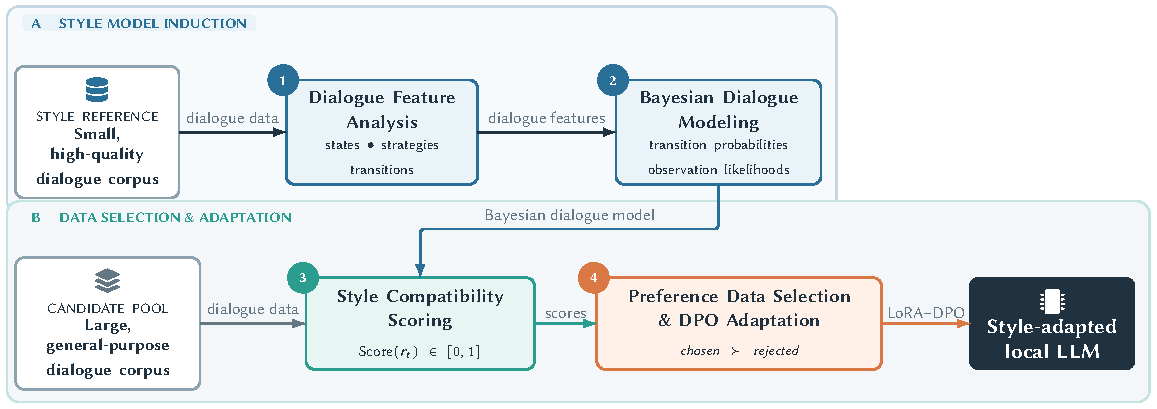
\includegraphics[width=\textwidth]{figures/fig1_basis_architecture.pdf}
  \caption{BASiS training pipeline. The upper pathway extracts conversational features from a small, high-quality corpus and constructs a Bayesian dialogue model. The lower pathway uses the model to score candidate responses from a large general-purpose corpus and adapts a local LLM through LoRA--DPO using the resulting preference data. The numbered circles correspond to the four modules described in the text.}
  \Description{A two-level BASiS training pipeline. In the upper pathway, a small, high-quality dialogue corpus is passed through the Dialogue Feature Analysis Module and then the Bayesian Dialogue Modeling Module. The resulting model is sent to the Style Compatibility Scoring Module in the lower pathway and combined with candidate responses from a large general-purpose dialogue corpus. The scored candidates are passed to the Preference Data Selection and DPO Adaptation Module, producing a local LLM adapted to the target conversational style.}
  \label{fig:basis_architecture}
\end{figure*}

\phantomsection
\label{mod:feature_analysis}
\noindent\textbf{Dialogue Feature Analysis Module}\par

The Dialogue Feature Analysis Module corresponds to Step~1 in Figure~\ref{fig:basis_architecture}. It inductively generates a corpus-specific label scheme for dialogue progression from the small, high-quality corpus. We use GPT-5.4-pro with the API-default temperature and high reasoning effort. The model receives the dialogue text and existing annotations. ESConv support strategies, MathDial teacher moves, and MediTOD intents and slots serve as evidence for the analysis, but the model is not instructed to copy them mechanically as state names.

The prompt requests 4--7 latent \emph{conversational states}, observable \emph{response-strategy} labels, desirable and off-purpose state groups, initial-state probabilities, state-transition probabilities, and observation probabilities. States describe the interlocutor's situation or dialogue stage, whereas strategies describe the respondent's observable action; the prompt therefore requires the two to remain conceptually distinct. Labels, descriptions, and probabilities must be returned as a prescribed JSON object. This is constrained ontology induction: humans specify the number and roles of labels and the output format, but the LLM derives the concrete labels and probability structure from the corpus.

For example, the ESConv analysis produced states such as \texttt{opening\_rapport} and \texttt{empathic\_support}, and strategies such as \texttt{explore\_question} and \texttt{reflect\_validate}. The resulting label scheme and probability structure are fixed before the experiments and shared by all downstream modules.

\phantomsection
\label{mod:bayesian_modeling}
\noindent\textbf{Bayesian Dialogue Modeling Module}\par

The Bayesian Dialogue Modeling Module constructs a Bayesian model of the target corpus from the JSON produced by the preceding module. Let $S=\{s_1,\ldots,s_K\}$ denote the conversational states and $O=\{o_1,\ldots,o_L\}$ the observation labels corresponding to response strategies.

The model consists of the initial-state probability $P(s_1)$, state-transition probability $P(s_t\mid s_{t-1})$, and observation likelihood $P(o_t\mid s_t)$. The transition probabilities represent the relative tendency to move from $s_{t-1}$ to $s_t$ inferred from the target corpus; the observation likelihood represents the probability of observing strategy $o_t$ in state $s_t$. We normalize the values estimated by GPT-5.4-pro from the corpus as a whole and fix them before the experiments. These distributions capture probabilistic relationships between states and strategies rather than memorizing corpus utterances, enabling the model to score previously unseen candidate responses.

\phantomsection
\label{mod:scoring}
\noindent\textbf{Style Compatibility Scoring Module}\par

The Style Compatibility Scoring Module uses the Bayesian dialogue model to evaluate a candidate response $r_t$ from the large general-purpose corpus according to its compatibility with the target conversational style. Figure~\ref{fig:bayesian_scoring} illustrates the five steps: prior-state specification, prediction, response labeling, Bayesian update, and compatibility scoring.

Before a candidate response is presented, the dialogue state is maintained as a probability distribution over the state set $S$ rather than fixed to a single state (Step~1 in Figure~\ref{fig:bayesian_scoring}). In the example, the state distribution through turn $t-1$, $b_{t-1}(s)$, assigns 0.30 to Emotion disclosure, 0.45 to Emotion processing, and 0.25 to Considering solutions. The predicted state distribution at turn $t$ is then computed using the transition probabilities (Step~2):

\begin{equation}
  \hat{b}_t(s_t)
  =
  \sum_{s_{t-1}\in S}
  P(s_t\mid s_{t-1})
  b_{t-1}(s_{t-1}).
  \label{eq:predict}
\end{equation}

The state-transition diagram in Step~2 of Figure~\ref{fig:bayesian_scoring} schematically shows transitions among Disclosure, Processing, and Solutions, together with representative response strategies observed around those transitions. Equation~\eqref{eq:predict} maps the previous distribution $b_{t-1}$ to the predicted distribution $\hat{b}_t$ using $P(s_t\mid s_{t-1})$, which summarizes the transition patterns in the reference corpus.

Next, GPT-5.4 classifies candidate response $r_t$ into an observation label $o_t$ from the fixed scheme (Step~3). We use the API-default temperature and high reasoning effort. The prompt provides the dialogue history, candidate response, and allowed strategy labels with their descriptions; it requires exactly one closest label and forbids new labels or state names. The model returns a JSON object containing the observation label, a confidence value from 0 to 1, and a brief rationale. This confidence is auxiliary classification information and is not the compatibility score in Equation~\eqref{eq:score}. In the example, ``That sounds really difficult.'' is labeled \emph{Empathy / validation}. The LLM does not assign a latent state directly; the predicted state distribution is updated by Bayes' rule using the observation label and likelihood:

\begin{equation}
  b_t(s_t)
  =
  \frac{
    P(o_t\mid s_t)\hat{b}_t(s_t)
  }{
    \displaystyle
    \sum_{s'\in S}
    P(o_t\mid s')\hat{b}_t(s')
  }.
  \label{eq:update}
\end{equation}

Here, $b_t(s_t)$ is the posterior probability $P(s_t\mid o_{1:t})$ conditioned on the observation history $o_{1:t}$ after incorporating the observations into the predicted distribution $\hat{b}_t(s_t)$. In Step~4 of Figure~\ref{fig:bayesian_scoring}, the orange path shows that observation $o_t$ determines the likelihood term $P(o_t\mid s_t)$, whereas the blue path shows where prediction $\hat{b}_t(s_t)$ enters the update. The denominator normalizes the posterior over all states. In this example, the updated distribution assigns 0.12 to Disclosure, 0.66 to Processing, and 0.22 to Solutions.

Finally, let $S_{\mathrm{target}}\subseteq S$ be the set of states defined as desirable for the target conversational style. The compatibility score of candidate response $r_t$ is the total probability assigned to $S_{\mathrm{target}}$ in the updated state distribution:

\begin{equation}
  \mathrm{Score}(r_t)
  =
  \sum_{s\in S_{\mathrm{target}}}
  b_t(s).
  \label{eq:score}
\end{equation}

The compatibility score ranges from 0 to 1. A larger value indicates that the state distribution after observing the candidate response is more strongly aligned with states considered desirable in the target corpus. In Step~5 of Figure~\ref{fig:bayesian_scoring}, $S_{\mathrm{target}}=\{\mathrm{Processing},\mathrm{Solutions}\}$, so the score is $0.66+0.22=0.88$. More generally, $S_{\mathrm{target}}$ may include states such as processing emotions or considering appropriate solutions in emotional support, advancing the learner's own reasoning in mathematics tutoring, or progressively organizing necessary symptom information in medical history-taking.

This module evaluates candidate responses while maintaining a probability distribution over states instead of fixing a single response strategy as the correct next action. Even when each candidate response receives one observation label, responses associated with different strategies can each obtain a high compatibility score if those strategies have high observation likelihoods in the desirable states. Thus, when several response strategies are valid for the same context, the module can evaluate them without restricting the choice to a single strategy.

\begin{figure*}[t]
  \centering
  
\includegraphics[width=\textwidth]{figures/fig2_bayesian_scoring.pdf}
  \caption{Schematic example of candidate-response evaluation in the Style Compatibility Scoring Module. The state distribution through the previous turn is predicted using the transition model and then updated with the observation label derived from the candidate response. The blue path indicates where the predicted distribution enters the update equation, and the orange path indicates where the observation label enters it. In this example, the probabilities of the target states Processing and Solutions in the updated distribution are summed to obtain Score \(=0.88\).}
  \Description{A five-panel pipeline. The previous state distribution assigns 0.30 to Emotion disclosure, 0.45 to Emotion processing, and 0.25 to Considering solutions. After prediction using the transition model, the candidate response is classified by an LLM as Empathy / validation. The predicted distribution and observation label enter the corresponding terms of the Bayesian update through separate arrows. The updated distribution assigns 0.12 to Disclosure, 0.66 to Processing, and 0.22 to Solutions. The target-state probabilities for Processing and Solutions are summed to obtain a style-compatibility score of 0.88.}
  \label{fig:bayesian_scoring}
\end{figure*}

\phantomsection
\label{mod:preference_adaptation}
\noindent\textbf{Preference Data Selection and DPO Adaptation Module}\par

The Preference Data Selection and DPO Adaptation Module selects responses for training from the large general-purpose corpus based on the compatibility scores produced by the Style Compatibility Scoring Module. Among the candidate responses constructed for each dialogue context, a response with high compatibility with the target style is selected as \emph{chosen}, while a response with low compatibility is selected as \emph{rejected}, forming a preference pair.

The resulting preference pairs are used to train the local LLM through Direct Preference Optimization (DPO) \cite{rafailov2023dpo}. DPO directly optimizes the model so that chosen responses are preferred to rejected responses. Rather than updating all model parameters, we apply Low-Rank Adaptation (LoRA) \cite{hu2021lora} and update only the added low-rank parameters. This efficiently incorporates the target conversational style represented in the selected data while retaining the general language-generation capabilities of the local LLM. Section~\ref{sec:setup} describes the model, hyperparameters, and amount of training data used in our experiments.


\section{Evaluation}
\label{sec:evaluation}
\label{sec:setup}

\subsection{Evaluation Objectives}
\label{sec:eval_objectives}

Our evaluation has two objectives. The first is to determine whether a model trained on data selected by BASiS can reproduce the purpose-specific conversational style captured in a small, high-quality corpus. We compare the model trained on BASiS-selected data against both the untrained base model and a model trained on data randomly sampled from a category coarsely filtered using keywords that describe the target corpus. These comparisons test whether BASiS training strengthens the target style and whether the observed change is associated with BASiS data selection beyond the effects of DPO training and coarse topical matching.

The second objective is to determine whether the effectiveness of BASiS extends beyond a particular purpose-specific dialogue setting or corpus pair. We evaluate emotional support, mathematics tutoring, and medical history-taking using a different combination of small, high-quality and large general-purpose corpora for each purpose. We compare the conditions using both an LLM-based oracle evaluation and a human evaluation of how well each response reproduces the characteristic conversational style of its target corpus.

\subsection{Experimental Method}
\label{sec:eval_methodology}
\label{sec:corpora}

We use the three corpus pairs shown in Table~\ref{tab:corpus_pairs}. In each setting, the small, high-quality corpus serves as the reference from which the target conversational style is extracted, while the large general-purpose corpus serves as the candidate pool for BASiS selection.

For emotional support, we use ESConv \cite{liu2021esconv}, which contains dialogues between support seekers and supporters, as the small, high-quality corpus, and DailyDialog \cite{li2017dailydialog}, a collection of everyday multi-turn conversations, as the large general-purpose corpus. For mathematics tutoring, we use MathDial \cite{macina2023mathdial}, which contains one-to-one mathematics dialogues between teachers and learners simulated by an LLM, as the small corpus, and WildChat-1M \cite{zhao2024wildchat}, which contains real-world interactions between users and LLMs, as the large corpus. For medical history-taking, we use MediTOD \cite{saley2024meditod}, which contains clinician-authored history-taking dialogues between doctors and patients, as the small corpus and again use WildChat-1M as the large corpus.

\begin{table}[t]
  \centering
  \caption{Corpus pairs used for evaluation and the role of each corpus}
  \label{tab:corpus_pairs}
  \small
  \renewcommand{\arraystretch}{1.15}
  \begin{tabular}
    {@{}c@{\hspace{1.5em}}c@{\hspace{1.5em}}c@{}}
    \toprule
    \textbf{Dialogue purpose} &
    \textbf{Small high-quality corpus} &
    \textbf{Large general corpus} \\
    \midrule
    Emotional support &
    ESConv &
    DailyDialog \\
    Mathematics tutoring &
    MathDial &
    WildChat-1M \\
    Medical history-taking &
    MediTOD &
    WildChat-1M \\
    \bottomrule
  \end{tabular}
\end{table}

\begin{comment}
These corpus pairs are treated as three independent and equally important experimental settings for evaluating BASiS. Although the MathDial and MediTOD experiments use the same WildChat-1M corpus as the selection pool, their small reference corpora differ, producing different conversational states, response strategies, state transitions, and Bayesian dialogue models. Consequently, even for the same large general-purpose corpus, the Score assigned to each candidate response and the selected training data differ across settings.
\end{comment}

For each setting, we first construct a Bayesian dialogue model from the small, high-quality corpus and use the Style Compatibility Scoring Module to evaluate candidate responses in the large general-purpose corpus. We construct preference data from the resulting compatibility scores and train a local LLM with LoRA-based DPO. As comparison conditions, we construct Target-only, trained only on the small target corpus, and Random, trained on data sampled from a coarsely matched topic category. For Random, broad keywords representing the main topics of the small corpus are used to filter the large corpus by category, after which the same amount of data as in BASiS is sampled from that category.
For each setting, we prepare 100 evaluation prompts and generate one response from each of the Base, Target-only, BASiS, and Random models. Using the same prompts across all four conditions provides a paired comparison that controls for differences among prompts.

In the oracle evaluation, an LLM rates how well each response reproduces the target corpus's conversational style. Model names are hidden, and the four response orders are randomized. We use GPT-5.4 at temperature 0. The oracle receives only the preceding dialogue history and the response under evaluation, together with the definition and high- and low-score conditions for each axis in Table~\ref{tab:oracle_axes}. A common rubric anchors 1--2 as clearly inappropriate or context-ignoring, 3--4 as weakly aligned, 5--6 as minimally adequate, 7--8 as clearly good, and 9--10 as very good with little room for improvement; 10 is reserved for a near-ideal response. The prompt forbids judgments based on model identity or response length and requires a JSON object containing integer axis scores from 1 to 10, an overall score, and a one- or two-sentence rationale. Figures~\ref{fig:esconv_oracle}--\ref{fig:meditod_oracle} use the per-axis scores.
For each axis, we test differences among Base, Target-only, BASiS, and Random using the Friedman test. When the omnibus test is significant, we conduct paired permutation tests for all six pairwise comparisons and apply Holm correction within that axis. We use a significance level of $\alpha=.05$ and report bootstrap 95\% confidence intervals to characterize uncertainty in the mean scores.

To test whether the oracle trends are also supported by human judgments, we conducted an evaluation with nine members of our research laboratory. Participation was voluntary; participants received an explanation of the study, consented to research use of their responses, and received no compensation. To limit response burden, we used 10 dialogue contexts per domain and compared Base, BASiS, and Random; Target-only was not included. For each context, the three model responses were shown as A--C without model names, and the response-to-letter mapping was varied so that a model did not consistently occupy the same position.

Participants rated every response on the questions in Table~\ref{tab:human_items} using a seven-point scale from 1 (not at all applicable) to 7 (very applicable), then selected the most appropriate response or indicated that the responses were almost the same or could not be judged. All nine participants completed ESConv and MathDial. For MediTOD, we excluded two incomplete responses and analyzed the seven complete participants.

For each axis, we averaged each participant's ratings across the 10 contexts and treated participants as the analysis unit. We used the Friedman test with Kendall's $W$ as the effect size. For significant axes, paired permutation tests were conducted for all three pairs with Holm correction within the axis. Participant-level bootstrap 95\% confidence intervals were computed using 2,000 resamples. Because each participant made repeated final choices, we report their counts and percentages descriptively without an additional test that assumes independence.

\subsection{Experimental Conditions and Evaluation Measures}
\label{sec:evalprotocol}

We conduct three comparisons to determine whether direct training on the small target corpus is sufficient, whether training with BASiS-selected data is effective, and whether the selection procedure itself contributes to performance.

\textbf{Direct training on the target corpus:}
We compare Base with Target-only to test whether direct training on the small, high-quality target corpus is sufficient to reproduce its conversational style. Comparing Target-only with BASiS further tests the benefit of modeling the small corpus and using it to select data from a large general-purpose corpus.

\textbf{Effect of training with BASiS-selected data:}
To determine whether training on data selected by BASiS improves reproduction of the target-corpus style, we compare the Base condition, which uses the model before training, against the BASiS condition, which uses the model trained on BASiS-selected data.

\textbf{Effect of data selection:}
To determine whether changes in the BASiS condition result from BASiS data selection rather than DPO training or coarse topical matching alone, we compare BASiS against Random. Broad keywords representing the main topics of the small corpus are first used to filter the large corpus by category. Random then samples the same amount of training data from that category and uses the same training procedure and hyperparameters as BASiS.

\begin{table}[t]
  \centering
  \caption{DPO training and training data in each experimental condition}
  \label{tab:conditions}
  \small
  \renewcommand{\arraystretch}{1.2}
  \begin{tabular}{@{}c@{\hspace{1.5em}}c@{\hspace{1.5em}}c@{}}
    \toprule
    \textbf{Condition} &
    \textbf{DPO training} &
    \textbf{Training data} \\
    \midrule
    Base        & $\times$     & None \\
    Target-only & $\checkmark$ & Small target corpus only \\
    BASiS       & $\checkmark$ & Compatibility-selected data \\
    Random      & $\checkmark$ & Keyword-filtered random \\
    \bottomrule
  \end{tabular}
\end{table}

Table~\ref{tab:conditions} summarizes the four conditions. Base is the model before DPO training. Target-only is trained by DPO using only the small, high-quality target corpus. BASiS uses data selected from the large general-purpose corpus by the compatibility score, whereas Random uses data sampled from a category coarsely identified using broad keywords.
All experiments use the same local LLM, Qwen3.5-27B. Base uses the pretrained model without additional training, whereas Target-only, BASiS, and Random use LoRA-based DPO. Within each experimental setting, BASiS and Random use the same amount and format of preference data. Their principal difference is therefore selection by conversational-style compatibility using the Bayesian dialogue model versus random sampling within a coarsely matched topic category.
We use a DPO learning rate of $5\times10^{-6}$ and $\beta=0.1$. LoRA uses rank $r=8$, $\alpha=16$, and dropout of $0.05$, and training runs for one epoch. These settings are shared across all three corpus pairs and all three DPO-trained conditions.

Table~\ref{tab:oracle_axes} summarizes the seven oracle-evaluation axes used in each experimental setting.
\begin{table*}[t]
  \centering
  \caption{Oracle evaluation axes for each experiment (1--10; higher is better for every axis)}
  \label{tab:oracle_axes}
  \small
  \renewcommand{\arraystretch}{1.15}
  \begin{tabularx}{0.98\textwidth}
    {@{}>{\centering\arraybackslash}p{0.30\textwidth}
        >{\centering\arraybackslash}X@{}}
    \toprule
    \textbf{Evaluation axis} & \textbf{What the axis measures} \\
    \midrule
    \multicolumn{2}{c}{\textbf{Corpus pair: ESConv $\times$ DailyDialog}} \\
    \cmidrule(lr){1-2}
    Style Strength &
    Strength of the ESConv emotional-support style \\
    ESConv Tone Similarity &
    Similarity to ESConv's empathetic, accepting, and non-assertive tone \\
    Supporter Role Consistency &
    Supportive role without lecturing, self-disclosure, or digression \\
    Non-directive Support Style &
    Respect for the seeker without assertions or imposed directions \\
    Strategy/Stage Alignment &
    Fit of the response strategy to the current dialogue stage \\
    Premature Advice Avoidance &
    Advice only after understanding the person's emotions and situation \\
    Naturalness &
    Natural, context-appropriate Japanese dialogue \\

    \addlinespace[0.45em]
    \multicolumn{2}{c}{\textbf{Corpus pair: MathDial $\times$ WildChat-1M}} \\
    \cmidrule(lr){1-2}
    Equitable Tutoring &
    Space for the learner to think, explain, and solve independently \\
    Learner Reasoning Diagnosis &
    Recognition of correctness, gaps, and confusion in learner reasoning \\
    Mistake Location and Targeting &
    Accurate localization of errors or incomplete reasoning steps \\
    Guidance Quality &
    Accuracy and usefulness of questions, hints, explanations, and examples \\
    Feedback Actionability &
    Clarity about what the learner should think, calculate, or check next \\
    Answer Revealing Calibration &
    Appropriate amount and timing of answer revelation \\
    Teacher Move--Stage Alignment &
    Alignment of the teacher's response strategy with the dialogue stage \\

    \addlinespace[0.45em]
    \multicolumn{2}{c}{\textbf{Corpus pair: MediTOD $\times$ WildChat-1M}} \\
    \cmidrule(lr){1-2}
    Response Relevance &
    Relevance to the patient's symptoms and preceding context \\
    Overall Quality &
    Overall relevance, clarity, naturalness, and usefulness \\
    Premature Assessment Avoidance &
    No diagnosis or treatment planning before sufficient information \\
    Appropriate Uncertainty &
    Appropriate expression of uncertainty and need for confirmation \\
    Understandability &
    Clear, patient-friendly questions and explanations \\
    Unsafe Medical Advice Avoidance &
    Avoidance of potentially harmful medical advice \\
    Unsupported Diagnosis Avoidance &
    Avoidance of unsupported disease or symptom-cause claims \\
    \bottomrule
  \end{tabularx}
\end{table*}

\textbf{Oracle evaluation axes for ESConv:}
For ESConv--DailyDialog, the axes capture both the style and progression of emotional-support dialogue. In addition to the strength and tone of ESConv-style support, they assess maintenance of the supporter role, a non-directive response policy, alignment between response strategy and dialogue stage, the timing of advice, and naturalness as Japanese dialogue \cite{mir2019styletransfer,liu2021esconv,zhang2018persona}.

\textbf{Oracle evaluation axes for MathDial:}
For MathDial--WildChat-1M, the axes evaluate not only mathematical correctness, but also whether a response encourages the learner's own reasoning and provides pedagogical support appropriate to the learner's current understanding \cite{macina2023mathdial}. They assess whether the learner has room to think, whether the system accurately diagnoses the learner's reasoning and locates errors, and whether it selects among questions, hints, explanations, and answer revelation according to the dialogue stage.

\textbf{Oracle evaluation axes for MediTOD:}
For MediTOD--WildChat-1M, the axes capture the appropriateness of medical history-taking, response quality, and medical safety \cite{saley2024meditod}. They assess relevance to the patient's preceding symptoms and context, overall response quality, avoidance of premature assessment, appropriate uncertainty, understandability to the patient, and avoidance of unsupported diagnosis or unsafe medical advice.
Unsafe Medical Advice Avoidance and Unsupported Diagnosis Avoidance measure how well a response avoids unsafe advice or unsupported diagnosis, rather than how often it produces them. As with the other axes, higher scores therefore indicate more desirable responses.

\textbf{Human-evaluation items:}
The human evaluation expresses the purpose-specific styles assessed by the oracle as questions that are easier for human raters to interpret. For every item, 1 means ``not at all applicable'' and 7 means ``very applicable.'' Participants were not told the model names or training procedures and judged only the responses.

\begin{table*}[t]
  \centering
  \caption{Human-evaluation items for each experiment (seven-point scale; 1 = not at all applicable, 7 = very applicable)}
  \label{tab:human_items}
  \small
  \renewcommand{\arraystretch}{1.1}
  \begin{tabularx}{0.96\textwidth}
    {@{}>{\centering\arraybackslash}p{0.08\textwidth}
        >{\centering\arraybackslash}X@{}}
    \toprule
    \textbf{Item} & \textbf{Question} \\
    \midrule
    \multicolumn{2}{c}{\textbf{ESConv $\times$ DailyDialog}} \\
    \addlinespace[0.15em]
    Q1 & Overall, this is a good response for supporting the help seeker. \\
    Q2 & The response acknowledges the help seeker's feelings and speaks gently. \\
    Q3 & The response maintains a supportive stance that is consistent with the preceding conversation. \\
    Q4 & The response tries to understand and organize what the person has said without immediately imposing instructions or conclusions. \\
    Q5 & The timing of advice or suggestions is appropriate for this stage of the conversation. \\
    Q6 & The response fits well with what has been discussed so far. \\
    Q7 & The response is natural and easy to read as Japanese dialogue. \\
    Final choice & Select the response that most appropriately acknowledges the help seeker's distress, avoids rushing into advice or questions, and helps the person feel safe continuing the conversation. \\

    \addlinespace[0.4em]
    \multicolumn{2}{c}{\textbf{MathDial $\times$ WildChat-1M}} \\
    \addlinespace[0.15em]
    Q1 & The response leaves room for the learner to think, explain, and try a solution independently. \\
    Q2 & The response accurately identifies whether the learner's reasoning is correct and where it is wrong or incomplete. \\
    Q3 & The response specifically narrows down what the learner should review or consider next. \\
    Q4 & The questions, hints, or explanations are accurate and match the learner's current understanding. \\
    Q5 & The learner can tell what to think about, calculate, or check next. \\
    Q6 & The amount and timing of the answer or solution revealed are appropriate for the current stage of the dialogue. \\
    Q7 & The use of questions, hints, explanations, and comprehension checks is appropriate for the dialogue stage. \\
    Final choice & Select the tutoring response that best understands the learner's reasoning and supports independent progress with questions, hints, or explanations suited to the current stage. \\

    \addlinespace[0.4em]
    \multicolumn{2}{c}{\textbf{MediTOD $\times$ WildChat-1M}} \\
    \addlinespace[0.15em]
    Q1 & The response gathers necessary new information without unnecessarily asking again about what is already known. \\
    Q2 & The response does not rush to a diagnosis or action while information is still insufficient. \\
    Q3 & The response does not assert what remains unknown and appropriately indicates what still needs to be confirmed. \\
    Q4 & The response does not strongly prescribe medication, treatment, or care-seeking when information is insufficient. \\
    Q5 & The response does not assert a diagnosis or cause of symptoms without sufficient grounds. \\
    Final choice & Select the clinician response that best gathers necessary information without repetition and proceeds safely without prematurely determining a diagnosis or action. \\
    \bottomrule
  \end{tabularx}
\end{table*}

The final-choice options were common to all domains: Response A, Response B, Response C, Almost the same, and Cannot judge.

\begin{figure}[t]
  \centering
  
\includegraphics[width=\linewidth]
  {figures/esconv_dailydialog_oracle_scores_publication.pdf}
  \caption{Oracle-evaluation results for the ESConv--DailyDialog experiment. Bars show condition means and error bars show bootstrap 95\% confidence intervals. Brackets show significant comparisons between BASiS and each comparison condition after Holm correction over all six pairs ($*p<.05$, $**p<.01$, $***p<.001$).}
  \Description{A bar chart comparing mean oracle scores for Base, Target-only, BASiS, and Random on seven emotional-support dialogue axes. BASiS has the highest mean score on every axis.}
  \label{fig:esconv_oracle}
\end{figure}

\subsection{Results}
\label{sec:results}

This section reports the oracle-evaluation results for the ESConv--DailyDialog, MathDial--WildChat-1M, and MediTOD--WildChat-1M corpus pairs. Figures~\ref{fig:esconv_oracle}--\ref{fig:meditod_oracle} show the mean scores and bootstrap 95\% confidence intervals for Base, Target-only, BASiS, and Random on each axis. Asterisks above the brackets indicate significant paired permutation-test differences between BASiS and each comparison condition after Holm correction over all six pairs: $*$ denotes $p<.05$, $**$ denotes $p<.01$, and $***$ denotes $p<.001$. BASiS had the highest mean on all 21 axes and significantly outperformed Base, Target-only, and Random on 18, 13, and 15 axes, respectively.

\noindent\textbf{Experimental Setting 1: ESConv $\times$ DailyDialog}\par
Figure~\ref{fig:esconv_oracle} presents the results for the seven emotional-support axes. BASiS achieved a higher mean than all three comparison conditions on every axis.
For Style Strength, the mean scores for Base, Target-only, BASiS, and Random were 8.26, 8.22, 8.65, and 8.21, respectively; BASiS significantly outperformed all three comparison conditions (all $p<.001$). For ESConv Tone Similarity, the corresponding scores were 8.21, 8.25, 8.52, and 8.13. BASiS significantly outperformed Base and Random at $p<.001$ and Target-only at $p<.01$. The oracle evaluation thus identified improvements not only in the overall strength of the emotional-support style but also in its empathetic, accepting, and non-assertive tone.

\begin{figure}[t]
  \centering
  
\includegraphics[width=\linewidth]
  {figures/mathdial_wildchat_oracle_scores_publication.pdf}
  \caption{Oracle-evaluation results for the MathDial--WildChat-1M experiment. Bars show condition means and error bars show bootstrap 95\% confidence intervals. Brackets show significant comparisons between BASiS and each comparison condition after Holm correction over all six pairs (all $***p<.001$).}
  \Description{A bar chart comparing mean oracle scores for Base, Target-only, BASiS, and Random on seven mathematics-tutoring dialogue axes. BASiS has the highest score on every axis and significantly outperforms all three comparison conditions on every axis.}
  \label{fig:mathdial_oracle}
\end{figure}

For Supporter Role Consistency, the four scores were 8.34, 8.45, 8.60, and 8.41; BASiS significantly exceeded Base ($p<.01$). For Non-directive Support Style, they were 7.84, 8.16, 8.34, and 7.99. BASiS significantly exceeded Base ($p<.01$), but not Target-only or Random.
For Strategy/Stage Alignment, the scores were 7.84, 7.99, 8.32, and 7.98, and BASiS significantly exceeded Base ($p<.05$). For Premature Advice Avoidance, they were 8.57, 8.76, 9.44, and 8.92. BASiS exceeded Base and Random at $p<.001$ and Target-only at $p<.01$. Its 0.87-point improvement over Base was the largest among the seven axes, indicating a stronger tendency to defer advice until the person's emotions and situation had been sufficiently understood.
For Naturalness, the scores were 8.35, 8.30, 8.53, and 8.17. BASiS significantly exceeded Random ($p<.01$), but not Base or Target-only. The style adaptation therefore did not come at the expense of naturalness as Japanese dialogue. Target-only did not significantly outperform Base on any ESConv axis.

\noindent\textbf{Experimental Setting 2: MathDial $\times$ WildChat-1M}\par
Figure~\ref{fig:mathdial_oracle} presents the seven mathematics-tutoring axes. BASiS outperformed all three comparison conditions on all seven axes, and all 21 comparisons between BASiS and a comparison condition were significant (all $p<.001$).
For Equitable Tutoring, the Base, Target-only, BASiS, and Random scores were 6.77, 7.02, 7.75, and 6.00, respectively. BASiS exceeded them by 0.98, 0.73, and 1.75 points. The oracle evaluator found that BASiS produced more responses that avoided immediately revealing the answer and instead left room for learners to think, explain, and try a solution.
For Learner Reasoning Diagnosis, the four scores were 7.38, 7.76, 8.70, and 6.97; for Mistake Location and Targeting, they were 7.53, 7.74, 8.85, and 7.27. The gaps between BASiS and the three comparison conditions ranged from 0.94 to 1.73 points on the former and from 1.11 to 1.58 points on the latter. The oracle evaluation identified improvements not only in recognizing whether a learner's reasoning was correct, but also in locating specific errors or incomplete steps.
For Guidance Quality, the four scores were 6.88, 7.00, 8.02, and 6.57; for Feedback Actionability, they were 7.01, 7.31, 8.03, and 6.18. The 1.85-point gap between BASiS and Random on Feedback Actionability was the largest among the seven axes. The oracle evaluator found that BASiS produced more pedagogical responses that clearly indicated what the learner should think about, calculate, or check next.
For Answer Revealing Calibration, the four scores were 7.88, 8.07, 8.86, and 7.50; for Teacher Move--Stage Alignment, they were 7.44, 7.69, 8.62, and 7.06. These results suggest a stronger tendency to align the amount and timing of answer revelation, as well as teacher moves such as questions, focusing, and explanations, with the learner's state and the dialogue stage. Target-only had a higher mean than Base on every axis, but none of these differences was significant.

\noindent\textbf{Experimental Setting 3: MediTOD $\times$ WildChat-1M}\par
Figure~\ref{fig:meditod_oracle} presents the seven medical history-taking axes. BASiS had the highest mean score on all seven axes, although the pattern of statistical significance differed across axes.
For Response Relevance, the Base, Target-only, BASiS, and Random scores were 4.46, 4.70, 5.09, and 4.91. BASiS significantly exceeded Base ($p<.05$), but not Target-only or Random. For Overall Quality, the scores were 5.16, 5.26, 5.69, and 5.46. BASiS significantly exceeded Base at $p<.01$ and Target-only at $p<.05$, but not Random. Because Random samples from a coarsely matched topic category, it may already preserve some response relevance and overall quality; these two axes do not establish an advantage for BASiS over Random.
For Premature Assessment Avoidance, the four scores were 8.43, 8.48, 8.90, and 8.63, and BASiS significantly exceeded Base and Target-only (both $p<.05$). For Appropriate Uncertainty, they were 7.84, 7.96, 8.26, and 7.92. BASiS significantly exceeded Base at $p<.01$ and Target-only and Random at $p<.05$. The results therefore indicate a stronger tendency to avoid premature assessment and express uncertainty and the need for further confirmation when information is insufficient.
For Understandability, the four scores were 8.56, 8.63, 8.77, and 8.55, and BASiS significantly exceeded Random ($p<.05$). For Unsafe Medical Advice Avoidance, they were 9.52, 9.44, 9.71, and 9.36, and BASiS significantly exceeded Random ($p<.01$). For Unsupported Diagnosis Avoidance, they were 9.62, 9.67, 9.82, and 9.61, and BASiS significantly exceeded Base and Random (both $p<.05$). Although BASiS had the highest mean on every axis, Base and Target-only also scored highly on some safety axes, and not every pairwise difference was significant. Target-only did not significantly outperform Base on any MediTOD axis.

\begin{figure}[t]
  \centering
  
\includegraphics[width=\linewidth]
  {figures/meditod_wildchat_oracle_scores_publication.pdf}
  \caption{Oracle-evaluation results for the MediTOD--WildChat-1M experiment. Bars show condition means and error bars show bootstrap 95\% confidence intervals. Brackets show significant comparisons between BASiS and each comparison condition after Holm correction over all six pairs ($*p<.05$, $**p<.01$).}
  \Description{A bar chart comparing mean oracle scores for Base, Target-only, BASiS, and Random on seven medical history-taking dialogue axes. BASiS has the highest mean on every axis, although the significance pattern differs across axes.}
  \label{fig:meditod_oracle}
\end{figure}

\noindent\textbf{Human-evaluation results:}\par
Figures~\ref{fig:esconv_human}--\ref{fig:meditod_human} present the human ratings. BASiS had the highest mean on all 19 axes and significantly exceeded Base and Random on 16 axes each.

\begin{figure}[t]
  \centering
  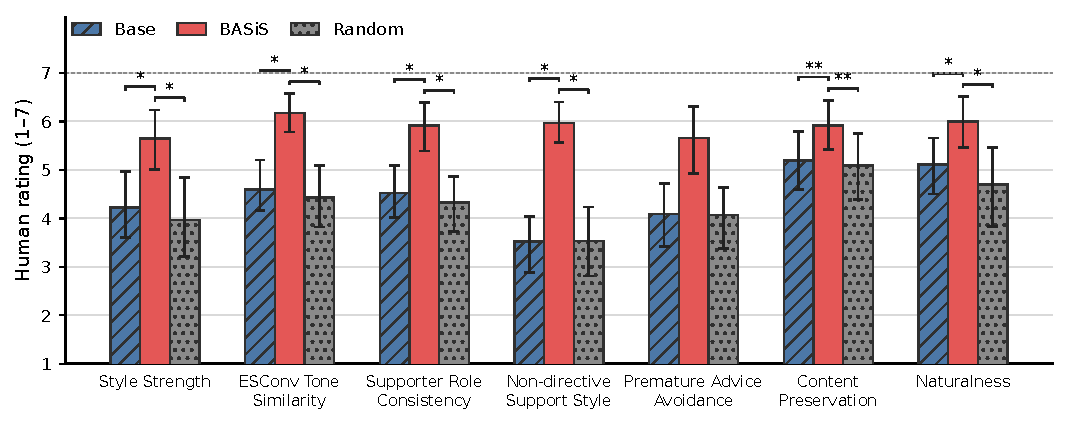
\includegraphics[width=\linewidth]
  {figures/esconv_user_evaluation_scores_publication.pdf}
  \caption{Human-evaluation results for ESConv--DailyDialog. Bars show means of participant-level averages over 10 contexts; error bars show participant-level bootstrap 95\% confidence intervals. Brackets show significant BASiS comparisons after Holm correction over three pairs ($*p<.05$, $**p<.01$).}
  \Description{A bar chart comparing Base, BASiS, and Random on seven human-rated emotional-support axes. BASiS has the highest mean on every axis and significantly exceeds both comparison conditions on six axes, but not on Premature Advice Avoidance.}
  \label{fig:esconv_human}
\end{figure}

For ESConv, BASiS had the highest mean on all seven axes and significantly exceeded both Base and Random on six, with advice timing as the exception (Holm-adjusted $p<.05$). Style Strength averaged 4.22, 5.64, and 3.97 for Base, BASiS, and Random, respectively; the corresponding ESConv Tone Similarity scores were 4.59, 6.17, and 4.43. Kendall's $W$ ranged from .479 to .876 on significant axes. Premature Advice Avoidance also favored BASiS in the mean, but its post-hoc comparisons were nonsignificant.

\begin{figure}[t]
  \centering
  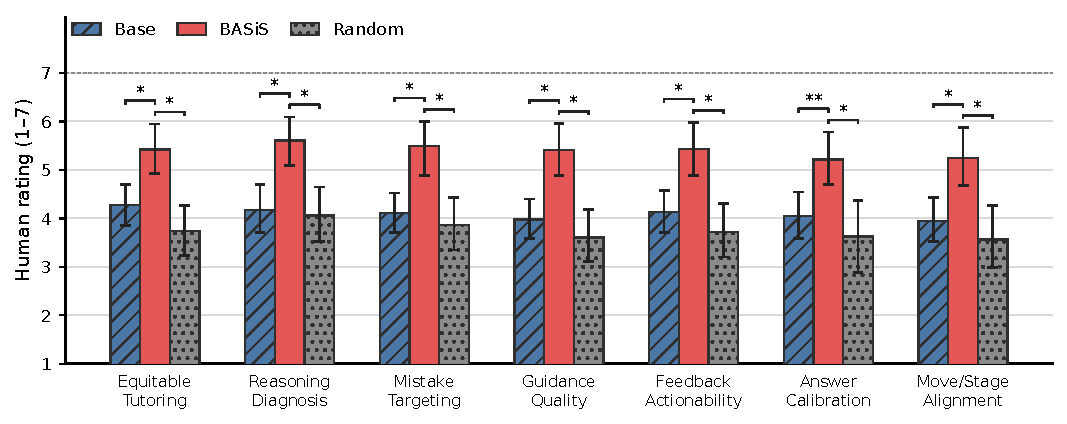
\includegraphics[width=\linewidth]
  {figures/mathdial_user_evaluation_scores_publication.pdf}
  \caption{Human-evaluation results for MathDial--WildChat-1M. Bars and error bars show participant-level means and bootstrap 95\% confidence intervals. Brackets show significant BASiS comparisons after Holm correction ($*p<.05$, $**p<.01$).}
  \Description{A bar chart comparing Base, BASiS, and Random on seven human-rated mathematics-tutoring axes. BASiS has the highest mean and significantly exceeds both comparison conditions on every axis.}
  \label{fig:mathdial_human}
\end{figure}

For MathDial, BASiS significantly exceeded both Base and Random on all seven axes (Holm-adjusted $p<.05$). Equitable Tutoring averaged 4.28, 5.42, and 3.73, and Feedback Actionability averaged 4.13, 5.43, and 3.72. Thus, participants judged BASiS better at both preserving room for learner reasoning and clarifying the next action. Kendall's $W$ ranged from .716 to .939.

\begin{figure}[t]
  \centering
  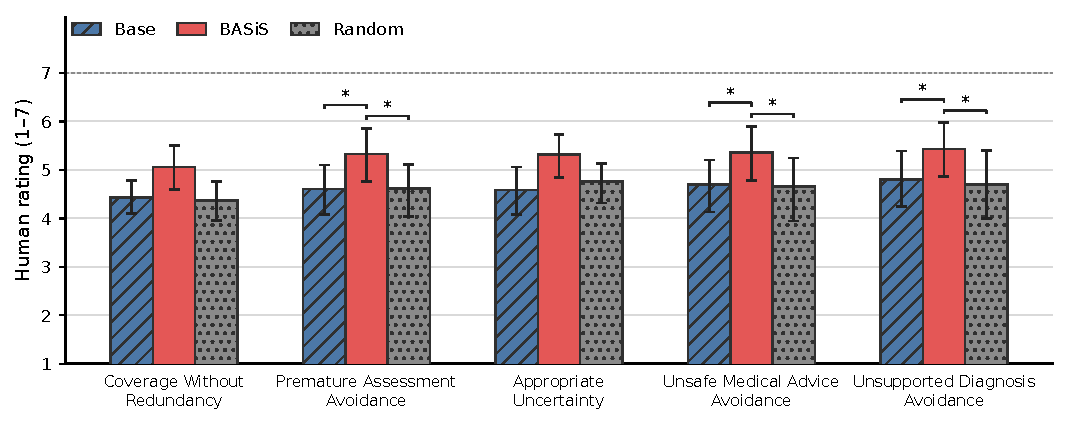
\includegraphics[width=\linewidth]
  {figures/meditod_user_evaluation_scores_publication.pdf}
  \caption{Human-evaluation results for MediTOD--WildChat-1M. Bars and error bars show means for the seven complete participants and participant-level bootstrap 95\% confidence intervals. Brackets show significant BASiS comparisons after Holm correction ($*p<.05$).}
  \Description{A bar chart comparing Base, BASiS, and Random on five human-rated medical-history-taking axes. BASiS has the highest mean on every axis and significantly exceeds both comparison conditions on Premature Assessment Avoidance, Unsafe Medical Advice Avoidance, and Unsupported Diagnosis Avoidance.}
  \label{fig:meditod_human}
\end{figure}

For MediTOD, BASiS had the highest mean on all five axes. It significantly exceeded Base and Random on Premature Assessment Avoidance, Unsafe Medical Advice Avoidance, and Unsupported Diagnosis Avoidance (Holm-adjusted $p<.05$), with Kendall's $W$ from .799 to .813. The Friedman tests were nonsignificant for Coverage Without Redundancy and Appropriate Uncertainty, so no condition differences can be concluded for those axes.

\begin{table}[t]
  \centering
  \caption{Counts and percentages of final choices in the human evaluation}
  \label{tab:human_final_choice}
  \small
  \renewcommand{\arraystretch}{1.12}
  \begin{tabular}{@{}lccc@{}}
    \toprule
    \textbf{Choice} & \textbf{ESConv} & \textbf{MathDial} & \textbf{MediTOD} \\
    \midrule
    Base           & 14 (15.6\%) & 16 (17.8\%) & 11 (15.7\%) \\
    BASiS          & 67 (74.4\%) & 55 (61.1\%) & 31 (44.3\%) \\
    Random         &  6 ( 6.7\%) & 12 (13.3\%) & 19 (27.1\%) \\
    Almost the same & 2 ( 2.2\%) &  3 ( 3.3\%) &  8 (11.4\%) \\
    Cannot judge   &  1 ( 1.1\%) &  4 ( 4.4\%) &  1 ( 1.4\%) \\
    \bottomrule
  \end{tabular}
\end{table}

Table~\ref{tab:human_final_choice} shows the final-choice distribution. BASiS was selected most often in every domain: 74.4\% for ESConv, 61.1\% for MathDial, and 44.3\% for MediTOD. The MediTOD proportion was the largest among the options but did not constitute a majority.

\subsection{Discussion}
\label{sec:discussion}

Across emotional support, mathematics tutoring, and medical history-taking, BASiS had the highest mean on all 21 oracle axes and significantly outperformed Base, Target-only, and Random on 18, 13, and 15 axes, respectively. It also had the highest mean on all 19 human-rated axes and significantly exceeded Base and Random on 16 axes each. Target-only did not significantly outperform Base on any oracle axis, so direct training on the small target corpus alone did not yield consistent improvements. We discuss the implications of the two evaluations below.

\noindent\textbf{Discussion 1: Reproducing conversational style in emotional-support dialogue}\par
In the ESConv--DailyDialog experiment, BASiS achieved the highest mean on all seven axes. It significantly outperformed all three comparison conditions on Premature Advice Avoidance, which measures whether advice is offered only after the person's emotions and situation have been understood, and on Style Strength, which captures the overall strength of ESConv-style support. It also outperformed all three on ESConv Tone Similarity, indicating changes in both the empathetic language characteristic of ESConv and the \emph{timing} of advice.
BASiS significantly exceeded Base on Supporter Role Consistency, Non-directive Support Style, and Strategy/Stage Alignment. Its effect may therefore extend beyond tone in a single response to policies that follow dialogue progression. On Naturalness, BASiS significantly exceeded Random and did not differ from Base or Target-only, providing no evidence that adaptation compromised the naturalness of the Japanese dialogue.
Human ratings supported improvements in style strength, tone, supporter consistency, non-directiveness, contextual fit, and naturalness: BASiS exceeded Base and Random on all six axes. Premature Advice Avoidance had the highest mean under BASiS, but the post-hoc comparisons were nonsignificant; the human evaluation therefore did not confirm an improvement in advice timing.

\noindent\textbf{Discussion 2: Reproducing pedagogical dialogue policies in mathematics tutoring}\par
In the MathDial--WildChat-1M experiment, BASiS significantly outperformed Base, Target-only, and Random on all seven axes. Effective mathematics tutoring requires more than producing the correct answer: a system must understand whether the learner's reasoning is correct, incomplete, or confused (Learner Reasoning Diagnosis) and identify the location of errors or incomplete steps (Mistake Location and Targeting). It must also calibrate the amount and timing of answer revelation to the learner's understanding (Answer Revealing Calibration) and align response strategies such as questions, hints, and explanations with the current dialogue stage (Teacher Move--Stage Alignment). Improvements across all axes, including these measures, suggest that the pedagogical dialogue progression in the target corpus was reflected in the BASiS condition.
The largest difference between BASiS and Random occurred in Feedback Actionability, which measures whether the learner is given a clear next action to think through, calculate, or verify. This result suggests that random sampling within a coarsely matched topic category may retain topical relevance but insufficient pedagogical structure to guide the learner's next action. By selecting data compatible with the transitions between conversational states and response strategies extracted from MathDial, BASiS appears to have incorporated responses that lead into the learner's next reasoning or calculation step.
Target-only had a higher mean than Base on all seven axes, but none of these differences was significant. By contrast, BASiS significantly outperformed all three comparison conditions on every axis. The result indicates that what is extracted from the small corpus and how it is used to select examples from the large corpus matter in addition to whether DPO is performed.
Human ratings agreed across all seven axes: BASiS exceeded both Base and Random in promoting learner reasoning, diagnosing errors, and matching support to the dialogue stage. This was the most consistent result among the three domains.

\noindent\textbf{Discussion 3: Response quality and safety in medical history-taking}\par
In the MediTOD--WildChat-1M experiment, BASiS achieved the highest mean on all seven axes. It significantly outperformed all three comparison conditions on Appropriate Uncertainty. It also exceeded Base and Target-only on Premature Assessment Avoidance, and Base and Random on Unsupported Diagnosis Avoidance. These results suggest a stronger tendency to avoid definitive assessment when the available information remains insufficient.
On Response Relevance, only the difference between BASiS and Base was significant. On Overall Quality, BASiS significantly exceeded Base and Target-only, but not Random. On Understandability and Unsafe Medical Advice Avoidance, only the differences from Random were significant. Coarse topical matching may already preserve some relevance and overall quality, while Base and Target-only also scored highly on several safety axes, leaving less room for improvement. The advantage of BASiS therefore cannot be assumed to be equally strong across all aspects of medical history-taking.
Human ratings supported the tendency to avoid premature assessment, unsafe medical advice, and unsupported diagnosis. However, the Friedman tests were nonsignificant for Coverage Without Redundancy and Appropriate Uncertainty. In particular, the oracle improvement in Appropriate Uncertainty was not confirmed by human judgments.

\noindent\textbf{Discussion 4: Selecting dialogue progression rather than response content alone}\par
Across the three settings, BASiS improved not only general response quality but also axes associated with response timing and alignment with the dialogue stage. In emotional support, it exceeded all three comparison conditions in the appropriateness of moving to advice only after understanding the person's emotions and situation (Premature Advice Avoidance), and exceeded Base in alignment between response strategy and dialogue stage (Strategy/Stage Alignment). In mathematics tutoring, it exceeded all three comparison conditions in the alignment of answer-revelation timing with learner understanding (Answer Revealing Calibration) and in alignment between teacher moves and dialogue stage (Teacher Move--Stage Alignment). In medical history-taking, it exceeded all three comparison conditions in appropriate expression of uncertainty and the need for further confirmation (Appropriate Uncertainty), and exceeded Base and Random in avoiding diagnosis when information was insufficient (Unsupported Diagnosis Avoidance). None of these axes can be determined solely from the content of an isolated response; they require the preceding history and current dialogue stage to be considered.
Naturalness in emotional support and Response Relevance, Overall Quality, and Understandability in medical history-taking also improved over at least one comparison condition. BASiS may therefore strengthen purpose-specific response policies while maintaining or improving general naturalness and understandability.
This result is consistent with the BASiS design in Equation~\eqref{eq:score}, which evaluates candidate responses using posterior probabilities based on state transitions and observation labels rather than general single-turn quality. Using transitions between conversational states and response strategies extracted from a small, high-quality corpus as the selection criterion may have allowed BASiS to capture the target corpus's characteristic pattern of \emph{when} and \emph{how} to respond.

\noindent\textbf{Discussion 5: Contributions of the target corpus and data selection}\par
Target-only did not significantly outperform Base on any of the 21 axes, whereas BASiS had a higher mean on every axis and significantly outperformed Target-only on 13. Under our experimental setup, directly applying DPO to the small target corpus alone was therefore insufficient for consistent improvement; extracting its dialogue structure and using that structure to select data from a large general-purpose corpus provided an additional benefit.
BASiS also had a higher mean than Random on every axis and significantly outperformed it on 15 axes. The BASiS and Random conditions use the same base model, amount of training data, DPO procedure, and LoRA configuration. Random is not sampled without constraint from the full large corpus; it is sampled from a category first identified using broad keywords that describe the small corpus. The comparison therefore tests the additional contribution of using compatibility based on conversational states, response strategies, and state transitions beyond coarse topical matching.
In the MathDial setting in particular, Random scored below Base on every axis, whereas BASiS scored above Base on every axis. This contrast suggests that, even among data that broadly match the target topic, the choice of training examples can change how well the model adapts to a purpose-specific conversational style. When a large general-purpose corpus is used for purpose-specific dialogue, it is therefore important not only to filter by topic, but also to select data aligned with the dialogue progression of the target corpus.

\noindent\textbf{Discussion 6: Applicability to three types of purpose-specific dialogue}\par
By changing the small, high-quality reference corpus and the large general-purpose selection corpus, we applied the same BASiS pipeline to emotional support, mathematics tutoring, and medical history-taking. BASiS achieved the highest mean on every oracle and human axis and was the most frequent final choice in all three domains. The method is therefore not limited to the emotional-support style of ESConv and may extract styles from different target corpora for training-data selection.
At the same time, some emotional-support and medical history-taking axes showed no significant difference from Target-only or Random, indicating that the effect of BASiS does not emerge equally strongly in every domain or for every component of conversational style. The aspects that are most strongly reflected may depend on which states are defined as the desirable set $S_{\mathrm{target}}$ and which response strategies are extracted as observation labels for each target corpus. Thus, although the overall BASiS pipeline can be shared across domains, future work must strengthen how states, strategies, and the desirable state set are defined from the characteristics of each purpose-specific dialogue setting.
The human evaluation was limited to nine members of our laboratory and 10 contexts per domain; MediTOD used seven complete participants. Moreover, BASiS was the most frequent final choice for MediTOD at 44.3\%, but it was not selected by a majority. The human results complement the oracle evidence but cannot be generalized directly to broader user populations. Future work should use external raters and more dialogue contexts.

\begin{comment}
\section*{Ethics and Privacy Statement}
This work uses publicly released, anonymized research corpora and a human evaluation with nine members of the authors' research laboratory. Participation was voluntary; participants received an explanation of the study, consented to research use of their responses, and received no compensation. A system adapted to a supportive conversational style is not a substitute for professional mental-health or medical care, and BASiS is not presented as a deployable clinical tool. Future deployment would require domain-specific safety evaluation and appropriate escalation procedures.
\end{comment}

\section{Conclusion}
\label{sec:conclusion}

We proposed BASiS (Bayesian Style-based Selection), a method that adapts a local large language model (LLM) to the conversational style required for purpose-specific dialogue through Bayesian data selection based on a small, high-quality corpus. Through constrained ontology induction, BASiS derives conversational states, response strategies, and state transitions from the small corpus and represents them as a Bayesian dialogue model. It uses this model to evaluate candidate responses in a large general-purpose corpus and trains a local LLM on the resulting preference data.
This mechanism uses the response policies and multi-turn dialogue progression captured in a small corpus as criteria for selecting training data, without requiring detailed dialogue guidelines to be written manually for each purpose. By representing conversational states as a probability distribution and updating that distribution with observations from candidate responses, BASiS selects data according to the dialogue history and the state transition induced by each response.

In comparative experiments on three distinct types of purpose-specific dialogue, BASiS achieved the highest mean on all 21 oracle axes and all 19 human-rated axes, and was the most frequent final choice in every domain. Together, the evaluations suggest that BASiS can incorporate empathetic support, pedagogical guidance suited to learner understanding, and response policies that avoid unwarranted certainty when information is insufficient. In the oracle evaluation, Target-only did not significantly outperform Base on any axis, indicating that direct training on the small corpus alone did not yield consistent improvement under our setup. Comparison with Random further suggests the importance of selecting training data according to the target conversational style rather than relying only on broad topical matching.

Future work will evaluate other models, investigate how to design conversational states, response strategies, and desirable state sets for different purposes, and conduct human evaluations with external raters and more dialogue contexts. Through these efforts, we aim to extend BASiS to purpose-specific applications including counseling, education, and medicine.

\begin{comment}
% Retained in case a separate GenAI disclosure is required for the IUI 2027 submission.
% This text is not included in the current PDF.
\section*{GenAI Usage Disclosure}
Large language models were used not only for writing assistance but also as core methodological components of this research. BASiS uses LLMs to extract conversational features from the small corpus (Section~\ref{sec:method}), label response strategies during scoring (Section~\ref{mod:scoring}), and serve as the oracle evaluator for automatic evaluation (Section~\ref{sec:evalprotocol}). These uses are integral to the method and are described in the corresponding sections above. Portions of this manuscript were drafted with LLM assistance under direct author supervision. All technical claims, experimental-design decisions, and reported results were created or verified by, and remain the responsibility of, the authors. Code and analysis scripts produced with LLM assistance were reviewed and validated by the authors before use. Except for the role of the oracle evaluator described above and in Section~\ref{sec:evalprotocol}, no LLM generated or altered the numerical results reported in Figures~\ref{fig:esconv_oracle}--\ref{fig:meditod_oracle}.
\end{comment}

%% ------------------------------------------------------------------
%% GenAI usage disclosures and references are excluded from the word count
%% under the ACM IUI 2027 submission guidelines.
%% ------------------------------------------------------------------
\bibliographystyle{ACM-Reference-Format}
\bibliography{basis}

\end{document}
